\documentclass[letterpaper, 10 pt, conference]{ieeeconf}  % Comment this line out if you need a4paper

%\documentclass[a4paper, 10pt, conference]{ieeeconf}      % Use this line for a4 paper

\IEEEoverridecommandlockouts                              % This command is only needed if 
                                                          % you want to use the \thanks command

\overrideIEEEmargins                                      % Needed to meet printer requirements.

% See the \addtolength command later in the file to balance the column lengths
% on the last page of the document

\usepackage{stmaryrd}

\newcommand{\todo}[1]{\textcolor{red}{\textbf{TODO:}} #1\\}

\newcommand{\RM}[1]{{\textcolor{red}{ \textbf{RM:} #1 $\clubsuit$ }}}
\newcommand{\RD}[1]{{\textcolor{blue}{ \textbf{RD:} #1 $\spadesuit$ }}}
\newcommand{\LF}[1]{{\textcolor{magenta}{ \textbf{LF:} #1 $\spadesuit$ }}}
\newcommand{\HH}[1]{{\textcolor{brown}{ \textbf{HH:} #1 $\spadesuit$ }}}

\newcommand{\mcomment}[1]{}

\DeclareMathOperator*{\sign}{sign}

\newcommand{\ie}{i.\,e.\xspace}
\newcommand{\as}{a.\,s.\xspace}
\newcommand{\wlg}{w.\,l.\,o.\,g.\xspace}
\newcommand{\wrt}{w.\,r.\,t.\xspace}

\newcommand{\mc}[1]{\mathcal{#1}}
\newcommand{\reals}{\mathbb{R}}
\newcommand{\nats}{\mathbb{N}}
\newcommand{\set}[1]{\ensuremath{\{ {#1} \}}}

\newcommand{\pctl}{PCTL\xspace}
\newcommand{\pctlstar}{PCTL$^*$\xspace}
\newcommand{\ctlstar}{CTL$^*$\xspace}
\newcommand{\atlstar}{ATL$^*$\xspace}


\newcommand{\atoms}{AP}
\newcommand{\true}{\mathsf{tt}}
\newcommand{\false}{\mathsf{ff}}
\newcommand{\probX}{\mathbb{P}}
\newcommand{\pquant}{\probX^{\quantifierTiny}}
\newcommand{\pforall}{\probX^{\forall}}
\newcommand{\pexists}{\probX^{\exists}}

\newcommand{\bfx}{\mathbf{x}}
\newcommand{\bfe}{\mathbf{e}}

\newcommand{\init}{\iota}
\newcommand{\pprog}{(\bfx,C)}
\newcommand{\mdp}{(S,\rho)}
\newcommand{\dtmc}{(S^\alpha,\rho^\alpha)}
\newcommand{\Distr}{\mathit{Distr}}
\newcommand{\Supp}{\mathit{Supp}}
\newcommand{\Prob}{\mathit{Prob}}
\newcommand{\Paths}{\mathsf{Paths}}

\newcommand{\Pree}{\mathsf{Pre}_{\exists}}
\newcommand{\Pref}{\mathsf{Pre}_{\forall}}

\newcommand{\Player}{\mathsf{Player}}


\newcommand{\sem}[1]{[\![#1]\!]}
\newcommand{\Safe}{\mathsf{Safe}}
\newcommand{\Reach}{\mathsf{Reach}}
\newcommand{\Outcome}{\mathsf{Outcome}}

\newcommand{\at}{\mathit{at}}
\newcommand{\inm}{\mathit{in}}
\newcommand{\preserve}{\mathit{preserve}}

\newcommand{\close}{\mathit{close}}
\newcommand{\far}{\mathit{far}}
\newcommand{\origin}{\mathit{origin}}

\newcommand{\abs}[1]{|#1|}
\newcommand{\inv}[1]{#1^{-1}}

\newcommand{\sched}{\alpha}
\newcommand{\event}{\mathcal{E}}
\newcommand{\pevent}{\omega}
\newcommand{\indicator}[1]{[#1]}
\newcommand{\SampleSpace}{\Omega}
\newcommand{\SigmaAlgebra}{\mathcal{F}}
\newcommand{\Measure}{\mu}
\newcommand{\ProbabilitySpace}{(\SampleSpace, \SigmaAlgebra, \Measure)}
\newcommand{\CondProb}[2]{\mathbb{P}(#1 \; | \; #2)}
\newcommand{\Exp}[1]{\mathbb{E}(#1)}
\newcommand{\CExp}[3][{}]{\mathbb{E}^{#1}(#2 \; | \; #3)}
\newcommand{\Set}[1]{\{#1\}}
\newcommand{\SetCond}[2]{\{#1 \;:\; #2\}}

\newcommand{\qual}{\mathsf{qualitative}}
\newcommand{\quan}{\mathsf{quantitative}}
\newcommand{\infst}{\mathsf{Inf}}

\newcommand{\probOr}{\otimes}
\newcommand{\porder}{\succ}

\newcommand{\quantifier}{\protect\rotatebox[origin=c]{180}{\ensuremath{\mathrm Q}}}
\newcommand{\quantifierTiny}{\protect\rotatebox[origin=c]{180}{\tiny\ensuremath{\mathrm Q}}}
\newcommand{\nqRule}[1]{\ensuremath{\textsc{#1}}}
\newcommand{\qRule}[3][\quantifierTiny]{\ensuremath{\nqRule{#3}^{#1}}_{#2}}
\newcommand{\qDiscRule}[3][\quantifierTiny]{\ensuremath{\overline{\nqRule{#3}}^{#1}}_{#2}}

\newtheorem{appxprop}{Proposition}
\newtheorem{appxlemma}{Lemma}

% colors 
\definecolor{darkred}{rgb}{0.7 0 0}
\definecolor{lightred}{rgb}{1 0.2 0}
\definecolor{ired}{rgb}{0.8 0.36 0.36}
\definecolor{darkgreen}{rgb}{0 0.5 0}
\definecolor{darkblue}{rgb}{0 0 0.7}
\definecolor{lightblue}{rgb}{0.390 0.582 0.925}
\definecolor{darkgray}{rgb}{0.3 0.3 0.3}
\definecolor{gray}{rgb}{0.5 0.5 0.5}
\definecolor{lightgray}{rgb}{0.90 0.90 0.90}
\newcommand\bluet[1]{\textcolor{darkblue}{#1}}
\newcommand\magentat[1]{\textcolor{magenta}{#1}}
\newcommand\redt[1]{\textcolor{darkred}{#1}}
\newcommand\greent[1]{\textcolor{darkgreen}{#1}}
\newcommand\oranget[1]{\textcolor{orange}{#1}}


\newcommand{\colorize}[4]{\only<#1>{#4}\only<#2>{\textcolor{#3}{#4}}}

\newcommand{\colthree}[7]{
\only<#1>{\textcolor{#4}{#7}}
\only<#2>{\textcolor{#5}{#7}}
\only<#3>{\textcolor{#6}{#7}}
}
\newcommand{\coltwo}[5]{
\only<#1>{\textcolor{#3}{#5}}
\only<#2>{\textcolor{#4}{#5}}
}

\tikzset{
    invisible/.style={opacity=0},
    emph/.style={color=magenta},
    alert/.style={color=red},
    anotherhl/.style={color=blue},
    bold/.style={very thick},
    emph on/.style={alt={#1{emph}{}}},
    alert on/.style={alt={#1{alert}{}}},
    anotherhl on/.style={alt={#1{anotherhl}{}}},
    arrow on/.style={alt={#1{->}{}}},
    bold on/.style={alt={#1{bold}{}}},
    visible on/.style={alt={#1{}{invisible}}},
    alt/.code args={<#1>#2#3}{%
        \alt<#1>{\pgfkeysalso{#2}}{\pgfkeysalso{#3}} % \pgfkeysalso doesn't change the path
        },
    }
    
\newcommand{\ifstmt}{\underline{\text{if}}\ }
\newcommand{\thenstmt}{\ \underline{\text{then}}\ }
\newcommand{\elsestmt}{\underline{\text{else}}\ }
\newcommand{\assertstmt}{\textbf{assert}}
\newcommand{\uniform}{\textbf{Uniform}}
\newcommand{\bernoulli}{\textbf{Bernoulli}}
\newcommand{\boolt}{\underline{\text{bool}}\ }
\newcommand{\intt}{\underline{\text{int}}\ }
\newcommand{\doublet}{\underline{\text{double}}\ }

\newcommand{\modc}[1]{\text{mc}(#1)}

\newcommand{\SharpSAT}{\#SAT}
\newcommand{\SharpSMT}{\#SMT}

\newcommand{\SharpP}{\#P}
    

\title{\LARGE \bf Synthesis of Surveillance Strategies via Belief Abstraction
}

\author{Suda Bharadwaj$^{1}$ and Rayna Dimitrova$^{2}$ and Ufuk Topcu$^{3}$% <-this % stops a space
%\thanks{*This work was not supported by any organization}% <-this % stops a space
%\thanks{$^{1}$Albert Author is with Faculty of Electrical Engineering, Mathematics and Computer Science, University of Twente, 7500 AE Enschede, The Netherlands {\tt\small albert.author@papercept.net}}%
%\thanks{$^{2}$Bernard D. Researcheris with the Department of Electrical Engineering, Wright State University, Dayton, OH 45435, USA {\tt\small b.d.researcher@ieee.org}}%
}


\begin{document}

\maketitle
\thispagestyle{empty}
\pagestyle{empty}

%%%%%%%%%%%%%%%%%%%%%%%%%%%%%%%%%%%%%%%%%%%%%%%%%%%%%%%%%%%%%%%%%%%%%%%%%%%%%%%%

\begin{abstract}
We study the problem of synthesizing a controller for a robot given an Linear Temporal Logic (LTL) specification, as well as a surveillance objective where it is required to maintain knowledge of the location of a moving adversarial target. We formulate this problem as a one-sided partial information game. We then reduce the partial information game to a full observation game using an abstracted belief set construction to avoid the exponential blow up of the state space. In order to ensure the surveillance requirement is satisfied, we allow it to be encoded in three different ways - a safety objective, a liveness objective, or both depending on the qualitative behavioural requirement for the user. This is then appended to the original specification and formulated as an assume guarantee problem for reactive synthesis on the abstract belief-set game. We then use a counterexample guided abstraction refinement scheme to refine the abstract belief states until a reactive synthesis controller is found.
\end{abstract}

%%%%%%%%%%%%%%%%%%%%%%%%%%%%%%%%%%%%%%%%%%%%%%%%%%%%%%%%%%%%%%%%%%%%%%%%%%%%%%%%

\section{INTRODUCTION}

Performing surveillance, that is, tracking the location of a target, has many applications. If the target is adversarial, this has applications  in patrolling and defense, especially in combination with other objectives, such as providing certain services or accomplishing a mission. Techniques for tracking non-adversarial but unpredictable targets have been proposed in settings like surgery to control cameras to keep a patient's organs under observation despite unpredictable motions of occluding obstacles. Mobile robots in airports have also been proposed to carry luggage for clients - requiring the robots to follow the human despite unpredictable motion and periodically losing vision of the target \cite{GonBanos02}. 

When dealing with a possibly adversarial target, a strategy for the surveying agent for achieving its objective can be seen as a strategy in a two-player game between the agent and the target. Since the agent may not always observe, or even know, the exact location of the target, surveillance is, by its very nature, a partial information problem.
It is thus natural to reduce surveillance strategy synthesis to computing a winning strategy for the agent in a two-player partial-information game against the target. Game-based models for related problems have been extensively studied in the literature. Notable examples include pursuit-evasion games~\cite{Chung2011}, patrolling games~\cite{Basilico12}, and graph-searching games~\cite{Kreutzer11}, where the problem is formulated as enforcing eventual detection, which is, in its essence a search problem -- once the target is detected, the game ends. For many applications, this formulation is too restrictive. Often, the goal is not to detect or capture the target, but to maintain certain level of information about its location over an unbounded (or infinite) time duration, or, alternatively, be able to obtain sufficiently precise information over and over again. In other cases, the agent has an additional objective, such as performing certain task, which might prevent him from capturing the target, but allow for satisfying a more relaxed surveillance objective.

In this paper, we study the problem of synthesizing strategies for enforcing \emph{temporal surveillance objectives}, such as the requirement to never let the agent's uncertainty about the target's location exceed a given threshold, or recapturing the target every time it escapes. To this end, we consider surveillance objectives specified in Linear Temporal Logic (LTL), equipped with basic surveillance predicates. This also allows for a seamless combination with other task specifications. Our computational model is that of a two-player game played on a finite graph, whose nodes represent the possible locations of the agent and the target, and whose edges model the possible (deterministic) moves between locations. The agent plays the game with partial information, as it can only observe the target when  it is in it's area of sight. The target, on the other hand, always has full information about the agent's location, even when the agent is not in sight. In that way, we consider a model with one-sided partial information, making the computed strategy for the agent robust against a potentially more powerful adversary. 

We formulate surveillance strategy synthesis as the the problem of computing a winning strategy for the agent in a partial-information game with a surveillance objective. There is a rich theory of partial information games with LTL objectives~\cite{DoyenR11,Chatterjee2013}, and it is well known that even for very simple objectives the synthesis problem is EXPTIME-complete~\cite{Reif84,BerwangerD08}. Moreover, all the standard algorithmic solutions to the problem are based on some form of \emph{belief set construction}, which transforms the imperfect-information game into a perfect-information game which may be exponentially larger, since the new set of states is the powerset of the original one. Thus, such approaches scale poorly in general, and are not applicable in most practical situations.

We address this problem by using \emph{abstraction}. We introduce an \emph{abstract belief set construction}, which underapproximates the information-tracking abilities of the agent (or, alternatively, overapproximates its belief, i.e., the set of positions it knows the target could be in). Using this construction we reduce surveillance synthesis to a two-player perfect-information game with LTL objective, which we then solve using off-the shelf reactive synthesis tools~\cite{EhlersR16}. Our construction guarantees that the abstraction is sound, that is, if a surveillance strategy is found in the abstract game, it corresponds to a surveillance strategy for the original game. If, on the other hand, such a strategy is not found, then the method automatically checks if this is due to the coarseness of the abstraction, in which case the abstract belief space is automatically refined. Thus, our method follows the general Counterexample Guided Abstraction Refinement (CEGAR)~\cite{ClarkeGJLV00} scheme, which has successfully demonstrated its potential in formal verification and reactive synthesis.

{\bf Contributions.} We make the following contributions:\\
(1) We propose a \emph{formalization of surveillance objectives} as temporal logic specifications, and frame surveillance strategy synthesis  as a partial-information reactive synthesis problem.\\
(2) We develop an \emph{abstraction method that soundly approximates} surveillance strategy synthesis, thus enabling the application of efficient techniques for reactive synthesis.\\
(3) We design procedures that \emph{automatically refine a given abstraction} in order to improve its precision when no surveillance strategy exists due to coarseness of the approximation.\\
(4) We evaluate our approach on different surveillance objectives (safety, liveness) combined with task specifications, and discuss the qualitatively different behaviour of the synthesized strategies for the different kinds of specifications.

{\bf Related work.}
While closely related to the surveillance problem we consider, pursuit-evasion games with partial information~\cite{Chung2011, Chin2010, Antoniades2003} formulate the problem as eventual detection, and do not consider combinations with other mission specifications. Other work, such as \cite{Vidal2002} and \cite{Kim2001}, incorporates additionally map building during pursuit in an unknown environment, but again solely for target detection.

Synthesis from LTL specifications~\cite{Pnueli1989}, especially from formulae in the efficient GR(1) fragment~\cite{Piterman2006}, has been extensively used in robotic planning (e.g.~\cite{wong2012,Kress2007}), but surveillance-type objectives, such as the ones we study here, have not been considered so far. Epistemic logic specifications~\cite{MeydenV98} can refer to the knowledge of the agent about the truth-value of logical formulas, but, contrary to our surveillance specifications, are not capable of expressing requirements on the size of the agent's uncertainty.

CEGAR has been developed for verification~\cite{ClarkeGJLV00}, and later for control~\cite{HenzingerJM03}, of LTL specifications. 
It has also been extended to infinite-state partial-information games~\cite{DimitrovaF08}, and used for sensor design~\cite{FuDT14}, both in the context of safety specifications. In addition to being focused on safety objectives, the refinement method in~\cite{DimitrovaF08} is designed to provide the agent with just enough information to achieve safety, and is thus not applicable to surveillance properties whose satisfaction depends on the size of the belief sets.

%Performing surveillance on an adversarial target, by its very nature, is a partial information problem. The agent may not always know the position of the target. However, surveillance in conjunction with a mission specification can be crucial in applications such as defense where it is important to keep track of (potentially hostile) targets whilst trying to satisfy a particular objective. 

%Since we are dealing with an adversarial target, a natural setting for formulating the problem is a two-player game. There are several flavours of partial information games that have been studied in the literature \cite{Chatterjee2013}, and in this paper we focus on turn-based one-sided partial-observation deterministic games on which we perform reactive control synthesis. It is one-sided as we allow the adversary full information on the location of the agent even if it is not in sight. 

%Related work in dealing with surveillance type objectives are pursuit-evasion games. There are several methods in formulating the problem such as enforcing eventual detection (at which point the game ends) \cite{Chen2010} or not allowing the target to move more than a certain distance away (\cite{keylist}). Partial information version of these games have also been studied in \cite{Antoniades2003,keylist} where it is shown that there is no existence theory for optimal solutions. However, these approaches treat the surveillance requirement as a search problem - once the target is detected the game is over. Work done by \cite{Vidal2002} and \cite{Kim2001} also include map building during pursuit but again with the sole purpose of target detection. Additionally, we do not enforce the requirement that the target(s) be detected. It is sufficient if we are able to bound our belief of the location below a user specified threshold for an infinite execution which allows for more richer, and more complex, behaviour than standard pursuit-evasion. So while there is work in pursuit-evasion games with partial information \cite{Chen2010} and even unknown environments \cite{Vidal2002}, these do not deal with additional mission specifications and also do not allow for the target to 'escape' and be recaptured as will be necessary in a setting with objectives beyond only capture.

%Our aim is to then synthesize a reactive controller that satisfies both the LTL specification as well as the surveillance objective. While it has been shown that for a general LTL specification, the synthesis problem is doubly exponential in the length of the formula \cite{Pnueli1989}, the work in \cite{Piterman2006} lays out a class of formulae called GR(1) that is $\mathcal{O}(N^3)$. This framework has been used extensively in robotic planning, for example in \cite{wong2012,Kress2007} and we do so here as well. We explicitly encode the surveillance requirement into the GR(1) formula to allow us to exploit the fast nature of GR(1) synthesis to solve a pursuit-evasion game. 

%However, we still have the issue of partial obsno ervability in our setting. The controller will need to choose actions even when the state of the adversary is not known. The standard approach to deal with the partial observability is by using a \emph{belief set construction} to reduce the problem to a full observability game \cite{Bertoli2006}. However, the number of belief states will be exponential in the number of states \cite{Rintanen2004} as the belief set construction takes a powerset of the number of states. In general, this scales poorly and is not usable in most practical situations. \todo{literature on other partial information reduction heuristics}. In this paper, to deal with this problem, we introduce \emph{abstract belief set construction}. This is an underapproximation of the true belief space and hence, if a controller is found, then we know a controller will exist in the fully refined belief space. If a controller is not found, we use counterexample guided abstract refinement (CEGAR) to split a belief set and the process is repeated. While CEGAR has been extensively used on abstract models for GR(1) reactive synthesis \cite{Alur2015,keylist}, to our knowledge it has not been used on belief state refinement in reducing a partial information game to a full information game. 

%The focus of this paper is to solve a modified pursuit-evasion game with additional LTL objectives in a partial information setting using reactive control synthesis. We propose a novel encoding of the surveillance requirement into the GR(1) specification to allow for assume guarantee control synthesis as well as a CEGAR approach in belief set construction in solving the partial information game. Our contributions in this paper are as follows:
%\begin{itemize}
%\item We encode the surveillance task as a safety specification which forces the agent to more closely follow the adversary in order to ensure the uncertainty (size of the belief set) on the location of adversary does not grow above the constraint.
%\item We also encode surveillance task as a liveness objective. This allows for the agent to be more relaxed in monitoring the location of the agent if it can ensure that it can see it again sometime in the future.
%\item We analyse the qualitatively different behaviour produced based on the specification type which allows the user to tailor the specification based on the requirements of the mission.
%\item Avoiding the state space blow up by abstract belief set construction and using counter example guided belief refinement for both the safety and liveness specification cases.
%\end{itemize}

%The rest of the paper is structured as follows. In section II we provide definitions and notations for partial-observation games and the encoding of the pursuit-evasion requirement as safety and liveness objectives in LTL. In section III, we present our belief set abstraction in reducing the partial information game to a full information and also detail the CEGAR process for the different types of objectives. In section IV we provide experiments on gridworlds along with a simulation in ROS using our proposed algorithm, and we conclude and provide future direction in section V. 



%%%%%%%%%%%%%%%%%%%%%%%%%%%%%%%%%%%%%%%%%%%%%%%%%%%%%%%%%%%%%%%%%%%%%%%%%%%%%%%%

\section{PARTIAL-OBSERVATION GAMES FOR SURVEILLANCE}
We begin by defining a formal model for describing surveillance strategy synthesis problems, in the form of a two player game between an agent and a target, in which the agent has only partial information about the target's location.

\subsection{Surveillance Game Structures}\label{sec:surveillance-games}
We define a \emph{surveillance game structure} to be  a tuple $G  = (\states,s^\init,\trans,\vis)$, with the following components:
\begin{itemize}
\item $\states = L_a \times L_t$ is the set of states, with $L_a$ the set of locations of the agent and $L_t$ the locations of the target;
\item $s^\init = (l_a^\init,l_t^\init)$ is the initial state;
\item $\trans \subseteq \states \times \states$ is the transition relation describing the possible moves of the agent and the target;
\item $\vis : \states \to \bools$ is a function that maps a state $(l_a,l_t)$ to $\true$ iff \emph{ position $l_t$ is in the area of sight of $l_a$}.
\end{itemize}


\begin{figure}
\subfloat[Surveilance arena \label{simple-grid}]{
%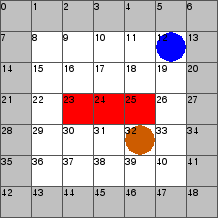
\includegraphics[scale=.33]{figs/7x7_safety.png}
\begin{tikzpicture}[scale=0.9]
\draw[step=0.5cm,color=gray] (-1.5,-1.5) grid (1,1);
\filldraw[fill=blue,draw=black] (+0.75,+0.75) circle (0.2cm);
\filldraw[fill=red,draw=black] (0,0) rectangle (-0.5,-0.5);
\filldraw[fill=red,draw=black] (-0.5,0) rectangle (-1,-0.5);
\filldraw[fill=red,draw=black] (0,0) rectangle (0.5,-0.5);
\filldraw[fill=blue!40!white,draw=black] (+0.75,+0.75) circle (0.2cm);
\filldraw[fill=orange!40!white,draw=black] (0.25,-0.75) circle (0.2cm);
\node at (-1.30,+0.75) {\tiny{0}};
\node at (-0.80,+0.75) {\tiny{1}};
\node at (-0.30,+0.75) {\tiny{2}};
\node at (0.20,+0.75) {\tiny{3}};
\node at (0.73,+0.75) {\tiny{4}};
\node at (-1.35,+0.25) {\tiny{5}};
\node at (-0.85,+0.25) {\tiny{6}};
\node at (-0.35,+0.25) {\tiny{7}};
\node at (0.25,+0.25) {\tiny{8}};
\node at (0.75,+0.25) {\tiny{9}};
\node at (-1.35,-0.25) {\tiny{10}};
\node at (-0.85,-0.25) {\tiny{11}};
\node at (-0.35,-0.25) {\tiny{12}};
\node at (0.25,-0.25) {\tiny{13}};
\node at (0.75,-0.25) {\tiny{14}};
\node at (-1.35,-0.75) {\tiny{15}};
\node at (-0.85,-0.75) {\tiny{16}};
\node at (-0.35,-0.75) {\tiny{17}};
\node at (0.25,-0.75) {\tiny{18}};
\node at (0.75,-0.75) {\tiny{19}};
\node at (-1.35,-1.25) {\tiny{20}};
\node at (-0.85,-1.25) {\tiny{21}};
\node at (-0.35,-1.25) {\tiny{22}};
\node at (0.25,-1.25) {\tiny{23}};
\node at (0.75,-1.25) {\tiny{24}};
\end{tikzpicture}
}
\hfill
\subfloat[Transitions from the initial state\label{fig:simple-transitions}]{
\begin{minipage}{5.0cm}
\vspace{-1.8cm}
{\fontsize{8}{10}\selectfont $\vis(4,18) = \false,\vis(4,17) = \false,$ $\vis(4,19) = \true, \vis(4,23) = \false$}

\smallskip

\begin{tikzpicture}[node distance=.75 cm,auto,>=latex',line join=bevel,transform shape,scale=0.75]
\node at (0,0) (s0) {$(4,18)$};
\node  [below left of=s0,yshift=-.5cm] (s3) {$(3,23)$};
\node  [below right of=s0,yshift=-.5cm] (s4) {$(9,17)$};
\node  [left of=s3,xshift=-.35cm] (s2) {$(3,19)$};
\node  [left of=s2,xshift=-.35cm] (s1) {$(3,17)$};
\node  [right of=s4,xshift=.35cm] (s5) {$(9,19)$};
\node  [right of=s5,xshift=.35cm] (s6) {$(9,23)$};

\draw [->] (s0) edge (s1.north);
\draw [->] (s0) edge (s2.north);
\draw [->] (s0) edge (s3.north);
\draw [->] (s0) edge (s4.north);
\draw [->] (s0) edge (s5.north);
\draw [->] (s0) edge (s6.north);
\end{tikzpicture}
\end{minipage}

}
\caption{A simple surveillance game on a grid arena. Obstacles are shown in red, the agent and the target are coloured in blue and orange respectively.}
\label{fig:simple-surveillance-game}
\vspace{-.7cm}
\end{figure}


The transition relation $T$ encodes the one-step move of both the target and the agent, where the target moves first and the agent moves second. For a state $(l_a,l_t)$ we denote with $\succs_t(l_a,l_t)$ the set of successor locations of the target:

$\succs_t(l_a,l_t) = \{l_t' \in L_t \mid \exists l_a'. ((l_a,l_t),(l_a',l_t')) \in T\}$.

We extend $\succs_t$ to sets of locations of the target by stipulating that the set $\post(l_a,L)$ consists of all possible successor locations of the target for states in $\{l_a\} \times L$. Formally, let $\post(l_a, L) = \bigcup_{l_t \in L}\succs_t(l_a,l_t)$.

For a state $(l_a,l_t)$ and a successor location of the target $l_t'$, we denote with $\succs_t(l_a,l_t,l_t')$ the set of successor locations of the agent, given that the target moves to $l_t'$: 

$\succs_a(l_a,l_t,l_t') = \{l_a' \in L_a \mid  ((l_a,l_t),(l_a',l_t')) \in T\}$.

We assume that for every $s \in \states$ there exists $s' \in \states$ such that $(s,s') \in T$, that is, from every state there is at least one move possible (this might be staying in the same state).

We also assume that when the target moves to an invisible location, its position does not influence the possible one-step moves of the agent. Formally, we require that if $\vis(l_a,l_t') = \vis(l_a,l_t'')=\false$, then $\succs_a(l_a,l_t,l_t') = \succs_a(l_a,l_t,l_t'')$. This assumption is natural in the setting when the agent can move in one step only to locations that are in its sight.

\begin{example}\label{ex:simple-surveillance-game}
Figure~\ref{fig:simple-surveillance-game} shows an example of a surveillance game on a grid.  The sets of possible locations $L_a$ and $L_t$ for the agent and the target both consist of the squares of the  grid. The transition relation $T$ encodes the possible one-step moves of both the agent and the target on the grid, and incorporates all desired constraints. For example, moving to an occupied location, or an obstacle, is not allowed. Figure~\ref{fig:simple-transitions} shows the possible transitions from the initial state $(4,18)$.

The function $\vis$ encodes straight-line visibility: a location $l_t$ is visible from a location $l_a$ if there is no obstacle on the straight line between them. Initially the target is not in the area of sight of the agent, but the agent knows the initial position of the target. However, once the target moves to one of the locations reachable in one step, in this case, locations $\{17,19,23\}$, this might no longer be the case. More precisely, if the target moves to location $19$, then the agent observes its location, but if it moves to one of the others, then the agent no longer knows its exact location. \qed
\end{example}




\subsection{Belief-Set Game Structures}

In surveillance strategy synthesis we need to state properties of, and reason about, the information which the agent has, i.e. its \emph{belief} about the location of the target. To this end, we can employ a powerset construction which is commonly used to transform a partial-information game into a perfect information one, by explicitly tracking the knowledge one player has as a set of possible states of the other player.

For a surveillance game structure $G  = (\states,s^\init,\trans,\vis)$ we define the corresponding \emph{belief-set game structure} $G_\belief  = (\states_\belief,s^\init_\belief,\trans_\belief)$ with the following components:
\begin{itemize}
\item $\states_\belief = L_a \times \beliefs$ is the set of states, with $L_a$ the set of locations of the agent, and $\beliefs$ the set of \emph{belief sets} describing information about the location of the target;
\item $s^\init_\belief = (l_a^\init,\{l_t^\init\})$ is the initial state;
\item $\trans_\belief \subseteq \states_\belief \times \states_\belief$ is the transition relation where $((l_a, B_t),(l_a', B_t')) \in \trans_\belief$ iff one of these holds:
\begin{itemize}
\item[(1)] $B_t' = \{l_t'\}$, $l_t' \in \post(l_a,B_t)$, $\vis(l_a,l_t') = \true$;
\item[(2)] $B_t' = \{l_t' \in \post(l_a,B_t)  \mid  \vis(l_a,l_t') = \false \}$.
%\item[(1)] $B_t' = \{l_t'\}$ for some $l_t'$ such that $\vis(l_a,l_t') = \true$ and
%there exists $l_t \in B_t$ with $((l_a,l_t),(l_a',l_t')) \in \trans$;
%\item[(2)] $\begin{array}{lll}
%B_t' = \{l_t' & \mid & \vis(l_a,l_t') = \false \text{ and } \\
%&& \exists l_t \in B_t.\ ((l_a,l_t),(l_a',l_t')) \in \trans\}. 
%\end{array}
%$
\end{itemize}
Condition (1) captures the successor locations of the target that can be observed from the agent's current position $l_a$. Condition (2), on the other hand, corresponds to the belief set consisting of all possible successor locations of the target not visible from position $l_a$. 
%\begin{itemize}
%\item[(1)] $B_t' = \{l_t'\}$ for some $l_t'$ such that $\vis(l_a,l_t') = \true$ and
%there exists $l_t \in B_t$ with $((l_a,l_t),(l_a',l_t')) \in \trans$;
%\item[(2)] there exists $l_t \in B_t$ such that $\vis(l_a,l_t) = \true$ and 
%$\begin{array}{lll}
%B_t' = \{l_t' & \mid & \vis(l_a,l_t') = \false \text{ and } \\
%&& ((l_a,l_t),(l_a',l_t')) \in \trans\};
%\end{array}
%$
%\item[(3)] $\begin{array}{lll}
%B_t' = \{l_t' & \mid & \vis(l_a,l_t') = \false \text{ and } \\
%&& \exists l_t \in B_t: \vis(l_a,l_t') = \false \\
%&& \text{and }  ((l_a,l_t),(l_a',l_t')) \in \trans\}.
%\end{array}
%$
%\end{itemize}
%The first condition captures the successor locations of the target that can be observed from the agent's current location $l_a$. Conditions (2) and (3) correspond to belief sets consisting of all possible successor locations of the target not visible from $l_a$. In (2) those are successors of a single possible current position $l_t$ of the target that is visible from $l_a$, while in (3) the belief consist of  successors of all positions in $B_t$ not visible from $l_a$.
\end{itemize}

%\noindent{\textit{Remark}} In our model, before making a move, the agent updates its belief about the target. Thus, the belief set at each step consists of the locations the target can be in, after it moves (since it moves first). Since the target moves again immediately after the agent moves, the agent does not update its belief after it completes its own move. We note that the results in this paper can be easily extended to the case when the belief is updated after each player's move by explicitly incorporating turn-switching in the model. We choose not do so, for the sake of keeping the presentation simple.

\begin{figure}
\begin{center}
\begin{tikzpicture}[node distance=.9 cm,auto,>=latex',line join=bevel,transform shape,scale=.8]
\node at (0,0) (s0) {$(4,\{18\})$};
\node  [below left of=s0,yshift=-.5cm,xshift=-.35cm] (s2) {$(3,\{17,23\})$};
\node  [below right of=s0,yshift=-.5cm,xshift=.35cm] (s3) {$(9,\{19\})$};
\node  [left of=s2,xshift=-1cm] (s1) {$(3,\{19\})$};
\node  [right of=s3,xshift=1cm] (s4) {$(9,\{17,23\})$};

\draw [->] (s0) edge (s1.north);
\draw [->] (s0) edge (s2.north);
\draw [->] (s0) edge (s3.north);
\draw [->] (s0) edge (s4.north);
\end{tikzpicture}
\end{center}

\caption{Transitions from the initial state in the belief-set game from Example~\ref{ex:simple-belief-game} where $\vis(4,17) = \vis(4,23) = \false$.}
\label{fig:simple-belief-game}
\vspace{-.5cm}
\end{figure}

\begin{example}\label{ex:simple-belief-game}
Consider again the surveillance game structure from Example~\ref{ex:simple-surveillance-game}. The initial belief set is $\{18\}$, consisting of the initial position of the target. After the first move of the target, there are two possible belief sets: the set $\{19\}$ resulting from the move to a location in the area of sight of the agent, and the belief set $\{17,23\}$ consisting of the two invisible locations reachable in one step from location $18$.
Figure~\ref{fig:simple-belief-game} shows the successor states of the initial state $(4,\{18\})$ in the belief-set game structure. \qed
\end{example}

Based on  $T_\belief$, we can define the functions $\succs_t : \states_\belief \to \mathcal{P}(\beliefs)$ and  $\succs_a : \states_\belief \times \beliefs \to \mathcal{P}(L_a)$ similarly to the corresponding functions defined for $G$. 

A \emph{run} of the belief-set game $G_\belief$ is an infinite sequence $s_0,s_1,\ldots$ of states in $\states_\belief$, where $s_0 = s_\abstr^\init$, and $(s_i,s_{i+1}) \in T_\belief$ for all $i \geq 0$. 

A \emph{strategy for the target in $G_\belief$} is a function $f_t: \states_\belief^+ \to \beliefs$ such that $f_t(\pi\cdot s) = B_t$ implies $B_t \in \succs_t(s)$ for every $\pi \in \states_\abstr^*$ and $s \in \states_\abstr$. That is, a strategy for the target suggests a move resulting in some belief set reachable from some location in the current belief.

A \emph{strategy for the agent in $G_\belief$} is a function $f_a : S^+ \times \beliefs \to S$ such that $f_a(\pi\cdot s,B_t) = (l_a',B_t')$ implies $B_t' = B_t$ and $l_a' \in \succs_a(s,B_t)$ for every $\pi \in \states_\abstr^*$, $s \in \states_\abstr$ and $B_t \in \beliefs$. Intuitively, a strategy for the agent suggests a move based on the observed history of the play and the current belief about the target's position.

The outcome of given strategies $f_a$ and $f_t$ for the agent and the target in $G_\belief$, denoted $\outcome(G_\belief,f_a,f_t)$, is a run $s_0,s_1,\ldots$ of $G_\belief$ such that for every $i \geq 0$, we have $s_{i+1} = f_a(s_0,\ldots,s_i,B_t^i)$, where $B_t^i = f_t(s_0,\ldots,s_i)$.

\subsection{Temporal Surveillance Objectives}
Since the states of a belief-set game structure track the information which the agent has, we can state and interpret surveillance objectives for the agent over the belief-set game structure. We now define the syntax and the semantics of the surveillance properties in which we are interested. 

We consider a set of \emph{surveillance predicates} $\SP = \{p_k \mid k \in \nats_{>0}\}$, where for $k \in \nats_{>0}$ we say that a state $(l_a,B_t)$ in the belief game structure satisfies $p_k$ (denoted $(l_a,B_t) \models p_k$) iff 
$|\{l_t \in B_t \mid \vis(l_a,l_t)  = \false \}| \leq k$. Intuitively, $p_k$ is satisfied by the states in the belief game structure where the size of the belief set does not exceed the threshold $k \in \nats_{>0}$.

We consider surveillance objectives expressed by formulas of linear temporal logic (LTL) over surveillance predicates.
% Since we are only interested in surveillance predicates that upper-bound the size of belief sets, we consider LTL formulas in negation normal form, in which we disallow the occurrence of negation in front of surveillance predicates.
 Our LTL surveillance formulas  are generated by the grammar
\[\varphi := p \mid \true \mid \false \mid \varphi \wedge \varphi \mid \varphi \vee \varphi \mid \LTLnext  \varphi  \mid \varphi \LTLuntil \varphi \mid \varphi \LTLrelease \varphi,\]

where $p \in \SP$ is a surveillance predicate, $\LTLnext$ is the \emph{next} operator, $\LTLuntil$ is the \emph{until} operator, and $\LTLrelease$ is the \emph{release} operator. We also define the derived operators 
\emph{finally}: $\LTLfinally \varphi = \true \LTLuntil \varphi$ and 
\emph{globally}: $\LTLglobally \varphi = \false \LTLrelease \varphi$.

LTL formulas are interpreted over (infinite) runs. If a run $\rho$ satisfies an LTL formula $\varphi$, we write $\rho \models \varphi$. The formal definition of LTL semantics can be found in~\cite{BaierKatoen08}. Here we informally explain the meaning of the formulas we use.

Of special interest will be surveillance formulas of the form $\LTLglobally p_k$, termed \emph{safety surveillance objective}, and $\LTLglobally\LTLfinally p_k$, called \emph{liveness surveillance objective}.
Intuitively, the safety surveillance formula $\LTLglobally p_k$ is satisfied if at each point in time the size of the belief set does not exceed $k$. The liveness surveillance objective $\LTLglobally\LTLfinally p_k$, on the other hand, requires that infinitely often this size is below or equal to $k$.

\begin{example}
We can specify that the agent is required to always know with certainty the location of the target as
$\LTLglobally p_1$.
A more relaxed requirement is that the agent's uncertainty never grows above $5$ locations, and it infinitely often reduces this uncertainty to at most $2$ locations: $\LTLglobally p_5 \wedge \LTLglobally\LTLfinally p_2$.
\qed
\end{example}


\subsection{Incorporating Task Specifications}
We can integrate LTL objectives not related to surveillance, i.e., \emph{task specifications}, by considering, in addition to $\SP$, a set $\AP$ of atomic predicates interpreted over states of $G$. In order to define the semantics of $p \in \AP$ over states of $G_\belief$, we restrict ourselves to predicates observable by the agent. 
Formally, we require that for $p \in \AP$, and states $(l_a,l_t')$ and $(l_a,l_t'')$ with $\vis(l_a,l_t')=\vis(l_a,l_t'')=\false$ it holds that $(l_a,l_t') \models p$ iff $(l_a,l_t'') \models p$. One class of such predicates are those that depend only on the agent's position.

\begin{example}
Suppose that $\mathit{at\_goal}$ is a predicate true exactly when the agent is at some designated goal location. We can then state that the agent visits the goal infinitely often while always maintaining belief uncertainty of at most $10$ locations using the LTL formula $\LTLglobally\LTLfinally \mathit{at\_goal} \wedge \LTLglobally p_{10}$.
\qed
\end{example}

\subsection{Surveillance Synthesis Problem}
A \emph{surveillance game} is a pair $(G,\varphi)$, where $G$ is a surveillance game structure and $\varphi$ is a surveillance objective. A \emph{winning strategy for the agent for $(G,\varphi)$} is a strategy $f_a$ for the agent in the corresponding belief-set game structure $G_\belief$ such that for every strategy $f_t$ for the target in $G_\belief$ it holds that $\outcome(G_\belief,f_a,f_t) \models \varphi$. Analogously, a \emph{winning strategy for the target for $(G,\varphi)$} is a strategy $f_t$ such that for every strategy $f_a$ for the target in $G_\belief$ it holds that $\outcome(G_\belief,f_a,f_t) \not\models \varphi$.

{\bf Surveillance synthesis problem:} Given a surveillance game $(G,\varphi)$, compute a winning strategy for the agent for $(G,\varphi)$, or determine that such a strategy does not exist.


It is well-known that two-player perfect-information games with LTL objectives over finite-state game structures are determined, that is exactly one of the players has a winning strategy. This means that, the agent does not have a winning strategy for a given surveillance game, if and only if the target has a winning strategy for this game. We thus refer to winning strategies of the target as \emph{counterexamples}.

%%%%%%%%%%%%%%%%%%%%%%%%%%%%%%%%%%%%%%%%%%%%%%%%%%%%%%%%%%%%%%%%%%%%%%%%%%%%%%%%

\section{BELIEF SET ABSTRACTION}
\subsection{Abstract Belief-Set Games}
For a partitioning $\part = \{Q_i\}_{i=1}^n$ of the set of states $\states$ in a game structure $G$ we define the function $\alpha_\part : \states \to \part$ such that for $s \in\states$ we let $\alpha_\part(s) = Q$ where $Q \in \part$ and $s \in Q$.
By abuse of notation we denote also with $\alpha_{\part} : \mathcal{P}(\states) \to \mathcal{P}(\part)$ the function defined by $\alpha_{\part}(S') = \{\alpha_\part(s) \mid s \in S'\}$.

Given a partitioning $\part = \{Q_i\}_{i=1}^n$ we define the game structure 
$G_\abstr  = (\states_\abstr,s^\init_\abstr,T_\abstr)$, where
\begin{itemize}
\item $\states_\abstr = L_a \times \mathcal P(\part) \cup L_a \times \big\{\{\{l_t\}\big\} \mid l_t \in L_t\}$ is the set of states with $L_a$ the locations of the agent and $\mathcal P(\part)$ the set of abstract states approximating belief sets
\item $s^\init_\abstr = (l_a^\init,\alpha_Q(\{l_t^\init\}))$ is the initial state,
\item $\trans_\abstr \subseteq \states_\abstr \times \states_\abstr$ is the transition relation such that $((l_a, A_t),(l_a', A_t')) \in T_\abstr$ if and only if some of the following four conditions is satisfied
\begin{itemize}

\item $A_t' = \{\{l_t'\}\}$ for $l_t' \in L_t$ with $\vis(l_a',l_t') = \true$, and 
$A_t = \{\{l_t\}\}$ and $((l_a,l_t),(l_a',l_t')) \in T$;
\item $A_t' = \{\{l_t'\}\}$ for $l_t' \in L_t$ with $\vis(l_a',l_t') = \true$, and
$A_t = \{B_1,\ldots,B_m\}$ with $m > 1$, and for some $B_i \in A_t$ and $l_t \in B_i$ we have $\vis(l_a,l_t) = \false$ and $((l_a,l_t),(l_a',l_t')) \in T$;


\item $A_t = \{\{l_t\}\}$ and $A_t' = \alpha_\part(B')$ where

$\begin{array}{lll}
B' = \{l_t' & \mid & \vis(l_a',l_t') = \false \text{ and }\\
&& ((l_a,l_t),(l_a',l_t')) \in T\}
\end{array}
$

\item $A_t = \{B_1,\ldots,B_m\}$ for some $m > 1$, and\\ $A_t' = \alpha_\part(B')$ where

$\begin{array}{lll}
B' = \{l_t' & \mid & \vis(l_a',l_t') = \false \text{ and }\\
&&\exists B \in A_t \exists l_t \in B.\; \vis(l_a,l_t) = \false\\ 
&&\phantom{\exists B \in A_t } \text{ and } ((l_a,l_t),(l_a',l_t')) \in T
\}
\end{array}
$
\end{itemize}
The first two conditions capture the successor locations of the target that can be observed from the agent's successor location, while the last two conditions  correspond to the belief set that consists of all possible successor locations of the target that are not visible from the corresponding successor location of the agent. Unlike in the definition of the belief-set game, here we distinguish different cases also with respect to the current state. In particular, in case the abstracted belief set is not a singleton set we take into account only the successors of transitions emanating from concrete states where the target location is not visible.

\end{itemize}

\Rayna{As in the definition of $T_\belief$ we also have the problem that $A_t'$ depends on $l_a'$ and not only on $(l_a,A_t)$.}

\begin{example}
\todo{abstract game structure for previous example}
\end{example}


\subsection{Soundness of Belief Set Abstraction}
In the construction of the abstract  game structure, we overapproximate the belief-set of the agent at each step. Since we consider surveillance predicates that impose upper bounds on the size of the belief, such an abstraction  gives more power to the target (and, dually less power to the agent).  This construction guarantees that the abstraction is \emph{sound}, meaning that an abstract strategy for the agent that achieves a surveillance objective corresponds to a winning strategy in the concrete game. This is stated in the following theorem.

\begin{theorem}
Let $G$ be a surveillance game structure, $\part = \{Q_i\}_{i=1}^n$ be an abstraction partition, and $G_\abstr = \alpha_\part(G)$. For every surveillance objective $\varphi$, if there exists a wining strategy for the agent in the abstract belief-set game $(\alpha_\part(G),\varphi)$, then there exists a winning strategy for the agent in the concrete surveillance game $(G,\varphi)$.
\end{theorem}

\paragraph{Choosing an abstraction partition} Choosing an 'appropriate' partition can result in a controller that can guarantee the surveillance specifications with fewer abstract belief states. However, choosing the abstraction partition is, in general, specific to the game environment. In section \ref{sec:experiments}, we present some examples with user specified partitions. If the abstraction is too coarse, the user can refine the abstract states with the help of counterexamples. The nature of these counterexamples for the classes of surveillance specifications presented in this papers are defined in the next section.

The refinement procedure can be automated (CEGAR), however, for space constraints we do not include the details in this paper. We remark that even with automated refinement, the choice of initial abstraction can make a difference in the final number of abstract states.



%%%%%%%%%%%%%%%%%%%%%%%%%%%%%%%%%%%%%%%%%%%%%%%%%%%%%%%%%%%%%%%%%%%%%%%%%%%%%%%%

\section{BELIEF REFINEMENT FOR SAFETY SURVEILLANCE OBJECTIVES}
\subsection{Counterexample Tree}
A winning strategy for the target in a game with safety surveillance objective can be naturally represented as a tree. 
An \emph{abstract counterexample tree} $\counterex_\abstr$ for $(G_\abstr,\LTLglobally p_k)$ is a finite tree,  whose nodes are labelled with states in $\states_\abstr$ such that the following conditions are satisfied:
\begin{itemize}
\item The root node is labelled with the initial state $s_\abstr^\init$;
\item A node is labelled with an abstract state  which violates $p_k$ (that is, $s_\abstr$ where $s_\abstr \not\models p_k$) iff it is a leaf;
\item The tree branches according to all possible transition choices of the agent. Formally, if an internal node $v$ is labelled with $(l_a,A_t)$, then there exists an $A_t'$  such that: (1) $((l_a,A_t),(l_a',A_t')) \in \trans_\abstr$ for some $l_a' \in L_a$, and (2) for every $l_a' \in L_a$ such that $((l_a,A_t),(l_a,A_t')) \in \trans_\abstr$, there is a child $v'$ of $v$ labelled with $(l_a',A_t')$.
\end{itemize}


A \emph{concrete counterexample tree} $\counterex_\belief$ for $(G_\belief,\LTLglobally p_k)$ is a finite tree with nodes labelled with states in $\states_\belief$ where:
\begin{itemize}
\item The root node is labelled with the initial state $s_\belief^\init$;
\item A node is labelled with a belief state which violates $p_k$ (that is, $s_\belief$ where $s_\belief \not\models p_k$) iff it is a leaf;
\item The tree branches according to all possible transition choices of the agent. Formally, if an internal node $v$ is labelled with $(l_a,B_t)$, then there exists a $B_t'$  such that: (1) $((l_a,B_t),(l_a',B_t')) \in \trans_\belief$ for some $l_a' \in L_a$, and (2) for every $l_a' \in L_a$ such that $((l_a,B_t),(l_a,B_t')) \in \trans_\belief$, there is a child $v'$ of $v$ labelled with $(l_a',B_t')$.
\end{itemize}

Due to the overapproximation of the belief-sets, not every counterexample in the abstract game corresponds to a winning strategy for the target in the original game.

An abstract counterexample $\counterex_\abstr$ in $(G_\abstr,\LTLglobally p_k)$ is \emph{concretizable} if there exists a concrete counterexample 
tree $\counterex_\belief$ in $(G_\belief,\LTLglobally p_k)$, which differs from $\counterex_\abstr$ only in the node labels, and each node labelled with $(l_a,A_t)$ in $\counterex_\abstr$ has label $(l_a, B_t)$ in $\counterex_\belief$ for which $B_t \subseteq \gamma(A_t)$.


\begin{figure}
\subfloat[Abstract counterexample tree\label{fig:simple-safety-counterex-abstr}]{
\begin{tikzpicture}[node distance=.9 cm,auto,>=latex',line join=bevel,transform shape,scale=.8]
\node at (0,0) (s0) {$(12,32)$};
\node  [below left of=s0,yshift=-.5cm,xshift=-.5cm] (s1) {$(11,\{Q_4,Q_5\})$};
\node  [below right of=s0,yshift=-.5cm,xshift=.5cm] (s2) {$(19,\{Q_4,Q_5\})$};

\draw [->] (s0) edge (s1.north);
\draw [->] (s0) edge (s2.north);
\end{tikzpicture}

}
\hfill
\subfloat[Concrete counterexample tree\label{fig:simple-safety-counterex-concr}]{
\begin{tikzpicture}[node distance=.9 cm,auto,>=latex',line join=bevel,transform shape,scale=.8]
\node at (0,0) (s0) {$(4,18)$};
\node  [below left of=s0,yshift=-.5cm,xshift=-.5cm] (s1) {$(3,\{17,23\})$};
\node  [below right of=s0,yshift=-.5cm,xshift=.5cm] (s2) {$(9,\{17,23\})$};

\draw [->] (s0) edge (s1.north);
\draw [->] (s0) edge (s2.north);
\end{tikzpicture}

}
\caption{Abstract and corresponding concrete counterexample trees for the surveillance game in Example~\ref{ex:simple-safety-counterex}.}
\label{fig:simple-safety-counterex}
\end{figure}

\begin{example}\label{ex:simple-safety-counterex}
Figure~\ref{fig:simple-safety-counterex-abstr} shows an abstract counterexample tree $\counterex_\abstr$ for the game $(\alpha_\part(G),\LTLglobally p_1)$, where $G$ is the surveillance game structure from Example~\ref{ex:simple-surveillance-game} and $\part$ is the abstraction partition from Example~\ref{ex:simple-abstr-game}. The counterexample corresponds to the choice of the target to move to one of the locations $31$ or $39$, which, for every possible move of the agent, results in an abstract state with abstract belief $B = \{Q_4,Q_5\}$ violating $p_1$.
A concrete counterexample tree $\counterex_\belief$ concretizing $\counterex_\abstr$ is shown in Figure~\ref{fig:simple-safety-counterex-concr}.
\qed
\end{example}

\subsection{Counterexample-guided refinement}
We now describe a procedure which determines whether an abstract counterexample for a safety surveillance objective is concretizable. This procedure essentially constructs the precise belief-sets corresponding to the abstract moves of the target that constitute the abstract counterexample.

\subsubsection{Forward belief-set propagation}
Given an abstract counterexample tree $\counterex_\abstr$ we annotate its nodes with states in $\states_\belief$ in a top-down manner as follows. 
The root node is labelled with $s_\belief^\init$. 
If $v$ is a node annotated with the belief set $(l_a,B_t) \in \states_\belief$, and  $v'$ is a child of $v$ in $\counterex_\abstr$ labelled with an abstract state $(l_a',A_t')$, then we annotate $v'$ with the belief set $(l_a',B_t')$, where 
$B_t' = \post(l_a,B_t) \cap \gamma(A_t')$. The counterexample analysis procedure based on this annotation is given in Algorithm~\ref{algo:cex-analysis-safety}.
If each of the leaf nodes of the tree is annotated with a belief set $(l_a,B_t)$ for which $(l_a,B_t) \not\models p_k$, then the new annotation gives us a concrete counterexample tree $\counterex_\belief$, which by construction concertizes $\counterex_\abstr$. Conversely, if there exists a leaf node annotated with $(l_a,B_t)$ such that $(l_a,B_t) \models p_k$, then we can conclude that the abstract counterexample tree $\counterex_\abstr$ is not concretizable and use the path from the root of the tree to this leaf node to refine the partition $\part$.
\Suda{We can move this algorithm to the appendix right? The process is described in the previous paragraph anyway.}
\begin{algorithm}[h]
\small
\KwIn{surveillance game $(G,\LTLglobally p_k)$,\newline abstract counterexample tree $\counterex_\abstr$}
\KwOut{a path $\pi$ in $\counterex_\abstr$ or {\sc concretizable}}

\smallskip

\While{there is a node $v$ in $\counterex_\abstr$ whose children\newline are not annotated with states in $\states_\belief$}{
 let $(l_a,B_t)$ be the state with which $v$ is annotated\;
 \ForEach{child $v'$ of $v$ labelled with $(l_a',A_t')$}{
 annotate $v'$ with $(l_a',\post(l_a,B_t)\cap\gamma(A_t'))$\;
}
}%
\leIf{there is a path $\pi$ in $\counterex_\abstr$ from the root to a leaf annotated with a sate $s_\belief$ where $s_\belief\models p_k$\newline}
{\KwRet{$\pi$;}}
{\KwRet{{\sc concretizable}}}

\smallskip


\caption{Analysis of abstract counterexample trees for games with safety surveillance objectives.}
\label{algo:cex-analysis-safety}
\end{algorithm}

\begin{theorem}
If Algorithm~\ref{algo:cex-analysis-safety} returns a path $\pi_\abstr$ in $\counterex_\abstr$, then $\counterex_\abstr$ is not concretizable, and $\pi_\abstr$ is a non-concretizable path, otherwise  $\counterex_\abstr$ is concretizable.
\end{theorem}

\begin{figure}
\begin{center}
\begin{tikzpicture}[node distance=.9 cm,auto,>=latex',line join=bevel,transform shape,scale=.75]
\node at (0,0) (s0) {$v_0:(12,32)$};
\node  [below left of=s0,yshift=-.5cm,xshift=-2.2cm] (s1) {$v_1:(11,\{Q_1\})$};
\node  [below right of=s0,yshift=-.5cm,xshift=2.2cm] (s2) {$v_2:(19,\{Q_1\})$};
\node  [below of=s1,yshift=-.5cm] (s4) {$v_4:(12,A)$};
\node  [below of=s2,yshift=-.5cm] (s7) {$v_7:(18,A)$};
\node  [left of=s4,xshift=-1cm] (s3) {$v_3:(10,A)$};
\node  [right of=s4,xshift=1cm] (s5) {$v_5:(18,A)$};
\node  [left of=s7,xshift=-1cm] (s6) {$v_6:(12,A)$};
\node  [right of=s7,xshift=1cm] (s8) {$v_8:(26,A)$};
\draw [->] (s0) edge (s1.north);
\draw [->] (s0) edge (s2.north);
\draw [->] (s1) edge (s3.north);
\draw [->] (s1) edge (s4.north);
\draw [->] (s1) edge (s5.north);
\draw [->] (s2) edge (s6.north);
\draw [->] (s2) edge (s7.north);
\draw [->] (s2) edge (s8.north);

\end{tikzpicture}

\end{center}
\vspace{-.2cm}
\caption{Abstract counterexample in Example~\ref{ex:simple-safety-unconcretizable}. The leaf nodes are labelled with the abstract belief set $A = \{Q_1,Q_2\}$.}
\label{fig:simple-safety-counterex-1}
\vspace{-.5cm}
\end{figure}

\begin{example}\label{ex:simple-safety-unconcretizable}
Let $G$ be the surveillance game structure from Example~\ref{ex:simple-surveillance-game}, and consider the surveillance game $(G,\LTLglobally p_5)$. 
Let $\part = \{Q_1,Q_2\}$ consist of the set $Q_1$, corresponding to the first two columns of the grid in Figure~\ref{simple-grid} and the set $Q_2$ containing the locations from the other three columns of the grid. Figure~\ref{fig:simple-safety-counterex-1} shows a counterexample tree $\counterex_\abstr$ in the abstract game $(\alpha_\part(G),\LTLglobally p_5)$. The analysis in Algorithm~\ref{algo:cex-analysis-safety} annotates node $v_1$ with the concrete belief set $\{17,23\}$, and the leaf node $v_3$ with the set $B = \{16,18,22\}$. Thus, this counterexample tree $\counterex_\abstr$ is determined to be unconcretizable and the partition $\part$ should be refined.\qed
\end{example}

When the analysis procedure determines that an abstract counterexample tree is unconcretizable, it returns path in the tree that corresponds to a sequence of moves that the size of the belief-set does not actually exceed the threshold, given that the target behaves in a way consistent with the abstract counterexample.  Based on this path, we can then refine the abstraction in order to precisely capture this information and thus eliminate this abstract counterexample.


\subsubsection{Backward partition splitting}
Consider a path $\pi_\abstr = v_0,\ldots, v_n$ in $\counterex_\abstr$ where $v_0$ is the root node and $v_n$ is a leaf. For each node $v_i$, let $(l_a^i,A_t^i) $ be the abstract state labelling $v_i$ in $\counterex_\abstr$, and let $(l_a^i,B_t^i)$ be the  belief set with which the node was annotated by the counterexample analysis procedure. We consider the case when $(l_a^n,B_t^n) \models p_k$, that is, $|\{l_t \in B_t^n \mid \vis(l_a,l_t) = \false\}| \leq k$.
Note that since $\counterex_\abstr$ is a counterexample we have $(l_a^n,A_t^n) \not \models p_k$, and since $k>0$, this means $A_t \in \mathcal{P}(\part)$.


We now describe a procedure to compute a partition $\part'$ that refines the current partition $\part$ based on the path $\pi_\abstr$. Intuitively, we split the sets that appear in $A_t^n$ in order to ensure that in the refined abstract game the corresponding abstract state satisfies the surveillance predicate $p_k$. We may have to also split sets appearing in abstract states on the path to $v_n$, as we have to ensure that earlier imprecisions on this path do not propagate, thus including more than the desired newly split sets, and leading to the same violation of $p_k$.

Formally, if $A_t^n = (l_a^n,\{B_{n,1},\ldots,B_{n,m_n}\})$, then we split some of the sets $B_{n,1},\ldots,B_{n,m_n}$ to obtain from $A_t^n$ a set $A_j' = \{B_{n,1}',\ldots,B_{n,m_n'}'\}$ such that
\[|\{l_t \in \gamma(C^n) \mid \vis(l_a^n,l_t) = \false\}| \leq k \text{, where}\] 
\[C^n = \{B_{n,i}' \in A_j' \mid B_{n,i}' \cap B_t^n \neq \emptyset\}.\]
This property intuitively means that if we consider the sets in $A'$ that have non-empty intersection with $B_t^n$, an abstract state composed of those sets will satisfy $p_k$. Since $(l_a^n,B_t^n)$ satisfies $p_k$, we can find a partition $\part^n \preceq \part$ that guarantees this property, as shown in Algorithm ~\ref{algo:refinement-safety}.
 
What remains, in order to eliminate this counterexample, is to ensure that only these sets are reachable via the considered path, by propagating this split backwards, obtaining a sequence of partitions $\part \succeq \part^n \succeq \ldots \succeq \part^0$ refining $\part$. 

Given $\part^{j+1}$, we compute $\part^j$ as follows. For each $j$, we define a set $C^j \subseteq \mathcal{P}(L_t)$ (for $j=n$, the set $C^n$ was defined above). Suppose we have defined $C^{j+1}$ for some $j \geq 0$, and $A_t^j = (l_a^j,\{B_{j,1},\ldots,B_{j,m_j}\})$. We split some of the sets $B_{j,1},\ldots,B_{j,m_j}$ to obtain from $A_t^j$ a set $A_j' = \{B_{j,1}',\ldots,B_{j,m_j'}'\}$ where there exists $C^j \subseteq A_j'$ with
\[\gamma(C^j) = \{l_t \in \gamma(A_t^j) \mid \post(l_a^j,\{l_t\}) \cap \gamma(A_t^{j+1}) \subseteq \gamma(C^{j+1})\}.\] 
Intuitively, this means that the new partition allows us to express precisely the set of states that do not lead to sets in $A_{j+1}'$ that we are trying to avoid. 
Again, the fact that an appropriate partition $\part$ can be computed follows from the choice of the leaf node $v_n$. 
The procedure for computing the partition $\part' = \part^0$ that refines $\part$ based on such a path $\pi_\abstr$ is formalized in Algorithm~\ref{algo:refinement-safety}.
\begin{example}
We continue with the unconcretizable abstract counterexample tree from Example~\ref{ex:simple-safety-unconcretizable}. We illustrate the refinement procedure for the path $v_0,v_1,v_3$. For node $v_3$, we split $Q_1$ and $Q_2$ using the set $B = \{16,18,22\}$, obtaining the sets $Q_1' = Q_1 \cap \{16,18,22\} = \{16\}$, $Q_2' = Q_1\setminus\{16\}$, $Q_3' = Q_2 \cap \{16,18,22\} = \{18,22\}$ and $Q_4' = Q_2 \setminus \{18,22\}$. We thus obtain a new partition $\part_{v_3} \preceq \part$. In order to propagate the refinement backwards (to ensure eliminating $\counterex_\abstr$) we compute the set of locations from which the target can move to a location in $Q_2'$ or $Q_4'$ that is not visible from location $2$. In this case, these are just the locations $18$ and $22$, which have already been separated from $Q_2$, so here backward propagation does not require further splitting.\qed
\end{example}


\begin{algorithm}[h]
\small
\KwIn{surveillance game $(G,\LTLglobally p_k)$, abstraction partition $\part$,\newline unconcretizable path $\pi = v_0,\ldots,v_n$ in $\counterex_\abstr$}
\KwOut{an abstraction partition $\part'$ such that $\part' \preceq \part$}

\smallskip

let $(l_a^j,A_t^j)$ be the label of $v_j$, and $(l_a^j,B_t^j)$ its annotation;
\begin{flalign*}
A  :=&  \{Q \cap B_t^n\mid Q \in A_t^n , Q \cap B_t^n \neq \emptyset \}\cup &\\
& \{Q \setminus B_t^n\mid Q \in A_t^n , Q \setminus B_t^n \neq \emptyset \};
\end{flalign*}

$\part' := (\part \setminus A_t^n )  \cup A$

$C := \{ Q\in A \mid Q \cap B_t \neq \emptyset\}$

\For{$j = n-1,\ldots,0$}{
\lIf{$A_t^j \in L_t$}{{\bf break}}
$B :=  \{l_t \in \gamma(A_t^j) \mid \post(l_a,\{l_t\}) \subseteq \gamma(C)\}$\;
\noindent
\begin{flalign*}
A  := &\{Q \cap B\mid Q \in A_t^j , Q \cap B \neq \emptyset \}\cup &\\
& \{Q \setminus B\mid Q \in A_t^j , Q \setminus B \neq \emptyset \};
\end{flalign*}


$\part' := (\part' \setminus A_t^j )  \cup A$

$C := \{ Q\in A \mid Q \cap B \neq \emptyset\}$
} 
\KwRet{$\part'$}

\smallskip

\caption{Abstraction partition refinement given an unconcretizable path in an  abstract counterexample tree.}
\label{algo:refinement-safety}
\end{algorithm}

Let $\part$ and $\part'$ be two counterexample partitions such that $\part' \preceq \part$. Let $\counterex_\abstr$ be an abstract counterexample  tree in $(\alpha_\part(G),\LTLglobally p_k)$. We define $\gamma_{\part'}(\counterex_\abstr)$ to be the set of abstract counterexample trees in $(\alpha_{\part'}(G),\LTLglobally p_k)$ such that $\counterex'_\abstr \in \gamma(\counterex_\abstr)$ iff $\counterex'_\abstr$ differs from $\counterex_\abstr$ only in the node labels and for every node in $\counterex_\abstr$ labelled with $(l_a,A_t)$, the corresponding node in $\counterex'_\abstr$ is labelled with an abstract state $(l_a,A_t')$ such that $\gamma(A_t') \subseteq \gamma(A_t)$.
 
The theorem below states the progress property (eliminating the considered counterexample) of Algorithm~\ref{algo:refinement-safety}.

\begin{theorem}If $\part'$ is the partition returned by Algorithm~\ref{algo:refinement-safety} for an unconcretizable abstract counterexample $\counterex_\abstr$ in $(\alpha_\part(G),\LTLglobally p_k)$, then $\gamma_{\part'}(\counterex_\abstr) = \emptyset$, and also $\gamma_{\part''}(\counterex_\abstr) = \emptyset$ for every partition $\part''$ where $\part'' \preceq \part'$.
\end{theorem}

\begin{example}\label{ex:simple-safety-realizability}
In the surveillance game $(G,\LTLglobally p_5)$, where $G$ is the surveillance game structure from Example~\ref{ex:simple-surveillance-game}, the agent has a winning strategy. After $6$ iterations of the refinement loop we arrive at an abstract game $(\alpha_{\part^*}(G),\LTLglobally p_5)$, where the partition $\part^*$ consists of $11$ automatically computed sets (as opposed to the $22$ locations reachable by the target in $G$), which in terms of the belief-set construction means $2^{11}$ versus $2^{22}$ possible belief sets in the respective games.

In the game $(G,\LTLglobally p_2)$, on the other hand, the agent does not have a winning strategy, and our algorithm establishes this after one refinement, after which, using a partition of size $4$,  it finds a concretizable abstract counterexample.
\qed
\end{example}

%%%%%%%%%%%%%%%%%%%%%%%%%%%%%%%%%%%%%%%%%%%%%%%%%%%%%%%%%%%%%%%%%%%%%%%%%%%%%%%%

\section{BELIEF REFINEMENT FOR LIVENESS SURVEILLANCE OBJECTIVES}
\subsection{Counterexample Graph}
The counterexamples for general surveillance properties are directed graphs, which may contain cycles. In particular, for a liveness surveillance property of the form $\LTLglobally\LTLfinally p_k$ each infinite path in the graph has a position such that, from this position on, each state on the path violates $p_k$. An \emph{abstract counterexample graph} for the abstract game $(G_\abstr,\LTLglobally\LTLfinally p_k)$ is a finite graph $\counterex_\abstr$ defined analogously to the abstract counterexample tree. The addition being that for each cycle $\rho = v_1,v_2,\ldots,v_n$ with $v_1 = v_n$ in $\counterex_\abstr$ that is reachable from $v_0$, every node $v_i$ in $\rho$ is labelled with state $s_\abstr^i$ where $s_\abstr^i \not\models p_k$.
%\begin{itemize}
%\item There exists a node $v_0$ of $\counterex_\abstr$ labelled with $s^\init_\abstr$.
%\item For each cycle $\rho = v_1,v_2,\ldots,v_n$ with $v_1 = v_n$ in $\counterex_\abstr$ that is reachable from $v_0$, every node $v_i$ in $\rho$ is labelled with state $s_\abstr^i$ where $s_\abstr^i \not\models p_k$.
%\item The graph branches according to all possible transition choices of the agent. Formally, if a node $v$ is labelled with $(l_a,A_t)$, then there exists an $A_t'$  such that: (1) $((l_a,A_t),(l_a',A_t')) \in \trans_\abstr$ for some $l_a' \in L_a$, and (2) for every $l_a' \in L_a$ such that $((l_a,A_t),(l_a,A_t')) \in \trans_\abstr$, there is a child $v'$ of $v$ labelled with $(l_a',A_t')$.
%\end{itemize}   

\begin{figure}
\begin{minipage}{0.2\textwidth}
\begin{center}
%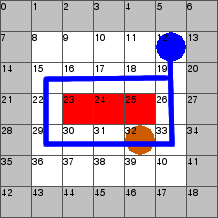
\includegraphics[scale=.33]{figs/7x7_liveness.png}
\begin{tikzpicture}
\draw[step=0.5cm,color=gray] (-1.5,-1.5) grid (1,1);
\filldraw[fill=blue,draw=black] (+0.75,+0.75) circle (0.2cm);
\filldraw[fill=red,draw=black] (0,0) rectangle (-0.5,-0.5);
\filldraw[fill=red,draw=black] (-0.5,0) rectangle (-1,-0.5);
\filldraw[fill=red,draw=black] (0,0) rectangle (0.5,-0.5);
\filldraw[fill=blue!40!white,draw=black] (+0.75,+0.75) circle (0.2cm);
\filldraw[fill=orange!40!white,draw=black] (0.25,-0.75) circle (0.2cm);
\draw[blue,thick] (-1.35,-0.75) rectangle (0.75,0.25);
\draw[blue,thick,->] (0.73,0.75) -> (0.75,0.25);
\node at (-1.30,+0.75) {\tiny{0}};
\node at (-0.80,+0.75) {\tiny{1}};
\node at (-0.30,+0.75) {\tiny{2}};
\node at (0.20,+0.75) {\tiny{3}};
\node at (0.73,+0.75) {\tiny{4}};
\node at (-1.35,+0.25) {\tiny{5}};
\node at (-0.85,+0.25) {\tiny{6}};
\node at (-0.35,+0.25) {\tiny{7}};
\node at (0.25,+0.25) {\tiny{8}};
\node at (0.75,+0.25) {\tiny{9}};
\node at (-1.35,-0.25) {\tiny{10}};
\node at (-0.85,-0.25) {\tiny{11}};
\node at (-0.35,-0.25) {\tiny{12}};
\node at (0.25,-0.25) {\tiny{13}};
\node at (0.75,-0.25) {\tiny{14}};
\node at (-1.35,-0.75) {\tiny{15}};
\node at (-0.85,-0.75) {\tiny{16}};
\node at (-0.35,-0.75) {\tiny{17}};
\node at (0.25,-0.75) {\tiny{18}};
\node at (0.75,-0.75) {\tiny{19}};
\node at (-1.35,-1.25) {\tiny{20}};
\node at (-0.85,-1.25) {\tiny{21}};
\node at (-0.35,-1.25) {\tiny{22}};
\node at (0.25,-1.25) {\tiny{23}};
\node at (0.75,-1.25) {\tiny{24}};
\end{tikzpicture}
\end{center}
\end{minipage}
\begin{minipage}{0.28\textwidth}
\caption{Agent locations on an (infinite) path in the abstract counterexample graph from Example~\ref{ex:simple-liveness-counterex}. In the counterexample graph, the first node is labelled with $(12,32)$, the second with $(19,\{Q_2\})$, and all other nodes with $(19,\{Q_1,Q_2\})$.}
\label{fig:simple-liveness-counterex}
\end{minipage}
\vspace{-.5cm}
\end{figure}

\begin{example}\label{ex:simple-liveness-counterex}
We saw in Example~\ref{ex:simple-safety-realizability} that in the safety surveillance game $(G,\LTLglobally p_2)$ the agent does not have a winning strategy. %This means, that the agent cannot ensure keeping at all times the uncertainty about the current position of the target to at most two positions.
We now consider a relaxed requirement, namely, the uncertainty drops to at most $2$ infinitely often, i.e., we consider the liveness surveillance game 
$(G,\LTLglobally \LTLfinally p_2)$.

Let $\part = \{Q_1,Q_2\}$ be the partition from Example~\ref{ex:simple-safety-unconcretizable}. %that is, $Q_1$, corresponds to the first two columns of the grid in Figure~\ref{simple-grid} and the set $Q_2$ contains the locations from the other three columns of the grid. 
Figure~\ref{fig:simple-liveness-counterex} shows an infinite path (in lasso form) in the abstract game $(\alpha_\part(G),\LTLglobally \LTLfinally p_2)$.  The figure depicts only the corresponding trajectory (sequence of positions) of the agent. The initial abstract belief set is $(4,18)$, the second node on the path is labeled with the abstract state $(9,\{Q_2\})$, and all other nodes on the path are labeled with abstract states of the form $(l_a,\{Q_1,Q_2\})$. As each abstract state in the cycle violates the surveillance predicate $p_2$, the path violates $\LTLglobally \LTLfinally p_2$. The same holds for all infinite paths in the abstract counterexample graph.
\qed
\end{example}

A \emph{concrete counterexample graph} $\counterex_\belief$ for the belief game $(G_\belief,\LTLglobally\LTLfinally p_k)$ is defined analogously. 

An abstract counterexample graph $\counterex_\abstr$ for the game $(G_\abstr,\LTLglobally\LTLfinally p_k)$ is \emph{concretizable} if there exists a counterexample
$\counterex_\belief$ in $(G_\belief,\LTLglobally \LTLfinally p_k)$, such that for each infinite path $\pi_\abstr = v_\abstr^0,v_\abstr^1,\ldots$ starting from the initial node of $\counterex_\abstr$ there exists an infinite path $\pi_\belief = v_\belief^0,v_\belief^1,\ldots$ in $\counterex_\belief$ staring from its initial node such that if $v_\abstr^i$ is labelled with $(l_a,A_t)$ in $\counterex_\abstr$, then the corresponding node $v_\belief^i$ in $\counterex_\belief$ is labelled with $(l_a,B_t)$ for some $B_t \in \mathcal{P}(L_t)$ for which $B_t \subseteq \gamma(A_t)$.


\subsection{Counterexample-guided refinement}
\subsubsection{Forward belief-set propagation}

To check if an abstract counterexample graph $\counterex_\abstr$ is concretizable, we construct a finite graph $\mathcal{D}$ whose nodes are labelled with elements of $\states_\belief$ and with nodes of $\counterex_\abstr$.
By construction we will ensure that if a node $d$ in $\mathcal D$ is labelled with $\langle(l_a,B_t),v \rangle$, where $(l_a,B_t)$ is a belief state, and $v$ is a node in $\counterex_\abstr$, then $v$ is labelled with $(l_a,A_t)$ in $\counterex_\abstr$, and $B_t \subseteq \gamma(A_t)$. 

Initially $\mathcal D$ contains a single node $d_0$ labelled with $\langle\{s_\belief^\init\},v_0\rangle$, where $v_0$ is initial node of $\counterex_\abstr$. Consider a node $d$ in $\mathcal D$ labelled with $\langle(l_a,B_t),v \rangle$. For every child $v'$ of $v$ in $\counterex_\abstr$, labelled with an abstract state $(l_a',A_t')$ we proceed as follows. We let ${B_t}' = \post(l_a,B_t) \cap \gamma(A_t')$. If there exists a node $d'$ in $\mathcal D$ labelled with $\langle (l_a',B_t'),v\rangle$, then we add an edge from $d$ to $d'$ in $\mathcal{D}$. Otherwise, we create such a node and add the edge. We continue until no more nodes and edges can be added to $\mathcal D$. The procedure is guaranteed to terminate, since both  the graph $\counterex_\belief$, and $\states_\belief$ are finite, and we add a node labelled $\langle s_\belief, v\rangle$ to $\mathcal D$ at most once.

If the graph $\mathcal D$ contains a reachable cycle (it suffices to consider simple cycles, i.e., without repeating intermediate nodes) $\rho = d_0,\ldots,d_n$ with $d_0 = d_n$ such that some $d_i$ is labelled with $(l_a,B_t)$ where $(l_a,B_t) \models p_k$, then we conclude that the abstract counterexample $\counterex_\abstr$ is not concretizable. If no such cycle exists, then $\mathcal D$ is a concrete counterexample graph for the belief game $(G_\belief,\LTLglobally\LTLfinally p_k)$. 

\begin{algorithm}[h] \small
\KwIn{surveillance game $(G,\LTLglobally\LTLfinally p_k)$, abstract counterexample graph $\counterex_\abstr$ with initial node $v_0$}
\KwOut{a path $\pi$ in a graph $\mathcal D$ or {\sc concretizable}}

\smallskip

graph $\mathcal D = (D,E)$ with nodes $D := \{d_0\}$ and edges $E := \emptyset$\;

annotate $d_0$ with $\langle s_\belief^\init, v_0\rangle$\; 

\SetKwRepeat{Do}{do}{while}

\Do{$\mathcal D \neq \mathcal D'$}{
$\mathcal D' := \mathcal D$\;
 \ForEach{node $d$ in $\mathcal D$ labelled with $\langle(l_a,B_t),v\rangle$}{
  \ForEach{child $v'$ of $v$ in $\counterex_\abstr$ labelled $(l_a',A_t')$}{
  $B_t' := \post(l_a,B_t)\cap\gamma(A_t')$\;
  \eIf{there is a node $d' \in D$ labelled with $\langle (l_a',B_t'),v'\rangle$}{add an edge $(d,d')$ to $E$}
  {add a node $d'$ labelled $\langle (l_a',B_t'),v'\rangle$ to $D$\;
  add an edge $(d,d')$ to $E$}
}
}
}
\leIf{there is a lasso path $\pi$ in $\mathcal D$ starting from $d_0$ such that some node in the cycle is annotated with $\langle s_\belief,v\rangle$ and $s_\belief\models p_k$\newline}
{\KwRet{$\pi$;}}
{\KwRet{{\sc concretizable}}}

\smallskip

\caption{Analysis of abstract counterexample graphs for games with liveness surveillance objectives.}
\label{algo:cex-analysis-liveness}
\end{algorithm}

\begin{example}\label{ex:simple-liveness-unconcretizable}
The abstract counterexample graph in the game $(\alpha_\part(G),\LTLglobally \LTLfinally p_2)$ discussed in Example~\ref{ex:simple-liveness-counterex} is not conretizable, since for the path in the abstract graph depicted in Figure~\ref{fig:simple-liveness-counterex} there exists a corresponding path in the graph $\mathcal D$ with a node in the cycle labelled with a set in $G_\belief$ that satisfies $p_2$. More precisely, the cycle in the graph $\mathcal D$ contains a node labelled with $(33,\{22\})$. Intuitively, as the agent moves from the upper to the lower part of the grid along this path, upon not observing the target, it can infer from the sequence of observations that the only possible location of the target is $22$. Thus, this paths is winning for the agent.
\qed
\end{example}

\begin{theorem}
If Algorithm~\ref{algo:cex-analysis-liveness} returns a path $\pi$ in the graph $\mathcal D$ constructed for $\counterex_\abstr$, then $\counterex_\abstr$ is not concretizable, and the infinite run in $G_\belief$ corresponding to $\pi$ satisfies $\LTLglobally\LTLfinally p_k$, otherwise  $\counterex_\abstr$ is concretizable.
\end{theorem}

\subsubsection{Backward partition splitting}

Consider a path in the graph $\mathcal{D}$ of the form $\pi = d_0,\ldots, d_n,d_0',\ldots,d_m'$ where $d_n = d_m'$, and where for some $0 \leq i \leq m$ for the label $(l_a^i,B_t^i)$ it holds that $(l_a^i,B_t^i) \models p_k$. Let 
$\pi_\abstr = v_0,\ldots, v_n,v_0',\ldots,v_m'$ be the sequence of nodes in $\counterex_\abstr$ corresponding to the labels in $\pi$. By construction of $\mathcal D$, $\pi_\abstr$ is a path in $\counterex_\abstr$ and $v_n = v_m'$. We apply the refinement procedure from the previous section to the whole path $\pi_\abstr$, as well as to the to the path-prefix $v_0,\ldots, v_n$.

Let $\part$ and $\part'$ be two counterexample partitions such that $\part' \preceq \part$. Let $\counterex_\abstr$ be an abstract counterexample graph in $(\alpha_\part(G),\LTLglobally\LTLfinally p_k)$. We define $\gamma_{\part'}(\counterex_\abstr)$ to be the set of abstract counterexample graphs in $(\alpha_{\part'}(G),\LTLglobally\LTLfinally p_k)$ such that for every infinite path $\pi$ in $\counterex_\abstr'$ there exists an infinite path $\pi$ in $\counterex_\abstr$ such that for every node in $\pi'$ labelled with $(l_a,A_t')$ the corresponding node in $\counterex_\abstr$ is labelled with an abstract state $(l_a,A_t)$ such that $\gamma(A_t') \subseteq \gamma(A_t)$.

\begin{theorem}If $\part'$ is the partition 
%returned by Algorithm~\ref{algo:refinement-liveness} 
obtained by refining $\part$ with respect to an uncocretizable abstract counterexample $\counterex_\abstr$ in $(\alpha_\part(G),\LTLglobally\LTLfinally p_k)$, then $\gamma_{\part'}(\counterex_\abstr) = \emptyset$, and also $\gamma_{\part''}(\counterex_\abstr) = \emptyset$ for every partition $\part''$ with $\part'' \preceq \part'$.
\end{theorem}

\begin{example}\label{ex:simple-liveness-refinement}
We refine the abstraction partition $\part$ from Example~\ref{fig:simple-liveness-counterex} using the path identified there, in order to eliminate the abstract counterexample. For this, following the refinement algorithm, we first split the set $Q_1$ into sets $Q_1' = \{22\}$ and $Q_2' = Q_1 \setminus \{22\}$, and let $Q_3' = Q_2$. However, since from some locations in $Q_2'$ and in $Q_3'$ the target can reach locations in $Q_2'$ and $Q_3'$ that are not visible from the agent's position $33$, in order to eliminate the counterexample, we need to propagate the refinement backwards along the path and split $Q_2'$ and $Q_3'$ further. With that, we obtain an abstraction partition with $10$ sets, which is guaranteed to eliminate this abstract counterexample. In fact, in this example this abstraction turns out to be sufficiently precise to obtain a winning strategy for the agent.
\qed
\end{example}

\subsection{Omega-regular surveillance and task objectives}
We have described refinement procedures for safety and liveness surveillance objectives. If we are given a conjunction of such objectives, we first apply the refinement procedure for safety, and if no path for which we can refine is found, we then apply the refinenment procedure for liveness. 

In the general case, we check if the counterexample contains a state for which the concrete belief is a strict subset of the abstract one. If this is not the case, then the counterexample is concretizable, otherwise we refine the abstraction to make this belief precise. In the special case when we have a conjunction of a surveillance and task specifications, we first refine with respect to the surveillance objective as described above, and if this is not possible, with respect to such a node. Since the set of states in the game is finite, the iterative refinement will terminate, either with a concretizable counterexample, or with a surveillance strategy.  


%\begin{itemize}
%\item $\LTLglobally p_k \wedge \LTLglobally\LTLfinally p_l$: first check concretizability of all paths in the graph to states violating the safety constraints, if one is not concretizable then done, if all are concretizable, then apply method for liveness
%\item general surveillance objectives: refine for some node where the true belief is more precise than the abstract one. not guaranteed to eliminate counterexample, but refinement loop guaranteed to still terminate since system is finite state and a proper split is done at each step. heuristics for identifying such nodes
%\item $\varphi_{\mathit{surveillance}} \wedge \varphi_{\mathit{task}}$  if surveillance is a conjunction of safety and liveness, then in sequence: safety, liveness, task; otherwise as previous item
%\item full specification language: as for general surveillance
%\end{itemize}



%%%%%%%%%%%%%%%%%%%%%%%%%%%%%%%%%%%%%%%%%%%%%%%%%%%%%%%%%%%%%%%%%%%%%%%%%%%%%%%%

\section{EXPERIMENTAL EVALUATION}
We present the results of our abstraction-based method for surveillance strategy synthesis on two case studies. We use slugs, a generalized reactive synthesis tool detailed in \cite{EhlersR16}. Simulations were run on a Intel i5-5300U 2.30 GHz CPU with 8 Gb of ram. 

\subsection{Liveness surveillance specification + task specification}
Figure~\ref{fig:case1} shows a gridworld divided into  'rooms'. The surveillance objective requires the agent to infinitely often know precisely the location of the target (either see it, or have a belief consisting of one cell). Additionally, it has to perform the task of patrolling (visiting infinitely often) the green 'goal' cell. Formally, the specification is $\LTLglobally\LTLfinally p_1 \wedge \LTLglobally\LTLfinally \mathit{goal}$. 


\begin{figure}
\centering
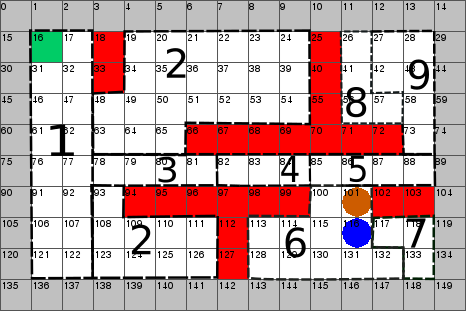
\includegraphics[scale=0.3]{text970.png}\caption{Gridworld with a computed partition of size $9$.}\label{fig:case1}
\vspace{-.5cm}
\end{figure}

%\begin{table}[h!]
%\begin{tabular}{c|c|c|c}
%& Not refined & Partially refined & Fully refined \\ \hline \hline
%Number of states & 104 & 616 & $2\times10^{31}$
%\end{tabular}
%\end{table}

Starting with an abstract game with 104 states generated by a partition with two elements, our refinement algorithm terminates after 5 iterations (with total running time of 821 s). The resulting partition $\mathcal{Q} = \{Q_1,...,Q_9 \}$ has $9$ elements shown as the numbered regions in Figure~\ref{fig:case1}. Thus, the final refined abstract game has $616$ abstract states ($2^9$ abstract belief states). In contrast, the belief-set game structure would have $2^{104}$ states, which is state-space size that state-of-the-art synthesis tools are not capable of handling.


%The refinement algorithm terminates after 5 iterations to produce the abstract partition  corresponding to the numbered sets in figure . There are 9 belief states which results in an additional $2^9 = 512$ states to the full observation game which is far lower than the full reduction which will be a power set of all 104 states.

A video simulation can be found at \url{http://goo.gl/YkFuxr}. Note the behaviour of the agent visiting the goal and then searching for the target. This will contrast with the behaviour under safety surveillance objectives which we look at next.

\subsection{Safety surveillance specification + task specification}
\begin{figure}
\centering
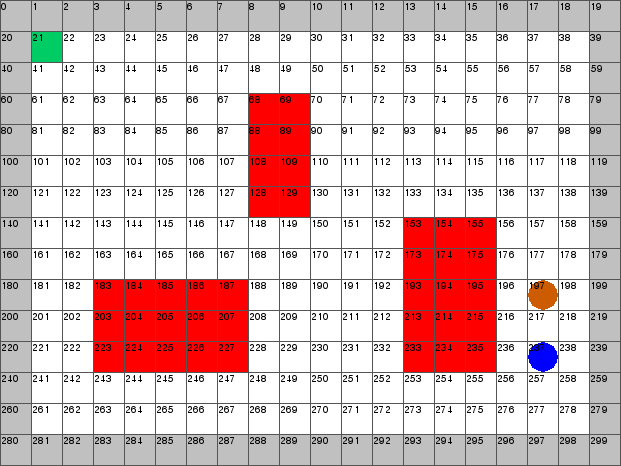
\includegraphics[scale=0.2]{case2.png}\caption{Gridworld representing an outdoor environment.}\label{fig:case2}
\vspace{-.5cm}
\end{figure}
Figure~\ref{fig:case2} depicts a gridworld of an 'outdoor' environment where the red blocks model buildings. 
In this setting, we enforce the safety surveillance objective $\square p_{30}$ in addition to infinitely often reaching the green cell. The formal specification is $\LTLglobally\LTLfinally p_{30} \wedge \LTLglobally\LTLfinally \mathit{goal}$. 
We used an abstraction generated by a partition of size 6, which was sufficiently precise to compute a surveillance strategy in 210 s. This demonstrates that even for larger grids, a coarse abstraction can be sufficient. Again, note that the precise belief-set game would have in the order of $2^{200}$ states.
 
We simulated the environment and the synthesized surveillance strategy for the agent in ROS. A video of the simulation can be found at \url{http://goo.gl/LyC1gQ}. Note the qualitative difference in behaviour compared to the previous example. In the case of liveness surveillance, the agent had more leeway to completely lose the target in order to reach its goal location, even though the requirement of reducing the size of the belief to $1$ is quite strict. Here, on the other hand, the safety surveillance objective, even with a large threshold of $30$, forces the agent to follow the target more closely, in order to prevent its belief from getting too large. The algorithm thus provides the ability to obtain qualitatively different behaviour as necessary for specific applications by combining these objective types. 

%\Suda{Not sure if we should keep this next part}
%\subsection{Discussion of behaviour}
%The difference in the behaviour in the case studies highlights the different use cases of the surveillance objectives. In more indoor settings or structured environments, a liveness surveillance objective is feasible as the agent can more easily search and find the target even if the belief grows very large. However, in outdoor environments this is harder to accomplish as the target has more room to hide. 

%%%%%%%%%%%%%%%%%%%%%%%%%%%%%%%%%%%%%%%%%%%%%%%%%%%%%%%%%%%%%%%%%%%%%%%%%%%%%%%%

\section{CONCLUSIONS}
We have presented a novel approach to solving a surveillance problem with information guarantees. We provided a framework that enables the  formalization of the surveillance synthesis problem as a two-player, partial-information game. We then presented a method to reason over the belief that the agent has over the target's location and specify formal surveillance requirements. The user can tailor the behaviour to their specific application by using a combination of safety and liveness surveillance objectives.

The benefit of the proposed framework is that it allows it leverages techniques successfully used in verification and reactive synthesis to develop efficient methods for solving the surveillance problem. There are several promising  avenues of future work using and extending this framework. Some of which currently being explored are the following;
\begin{itemize}
\item Synthesizing distributed strategies for multi-agent surveillance in a decentralized manner. These compositional synthesis methods avoid the blow up of the state space that occurs in centralized synthesis procedures as the number of surveillance agents grow.
\item Incorporating static sensors or alarm triggers for the mobile agent(s) to coordinate with.
\item Allowing for sensor models to include uncertainty and detection errors while still providing surveillance guarantees.

\end{itemize}

%%%%%%%%%%%%%%%%%%%%%%%%%%%%%%%%%%%%%%%%%%%%%%%%%%%%%%%%%%%%%%%%%%%%%%%%%%%%%%%%

\section*{APPENDIX}

%%%%%%%%%%%%%%%%%%%%%%%%%%%%%%%%%%%%%%%%%%%%%%%%%%%%%%%%%%%%%%%%%%%%%%%%%%%%%%%%

\section*{ACKNOWLEDGMENT}


%%%%%%%%%%%%%%%%%%%%%%%%%%%%%%%%%%%%%%%%%%%%%%%%%%%%%%%%%%%%%%%%%%%%%%%%%%%%%%%%
%\bibliographystyle{IEEEtran}
%\bibliography{IEEEabrv,main}

\end{document}
